\section{Case Study: RMSNorm}
\label{sec:case2}

In this section, we use root mean square layer normalization (RMSNorm)~\cite{zhang2019rootmeansquarelayer} as a case study to demonstrate the advantages of the \graph representation and \sys's superoptimization approach.
RMSNorm is a widely used normalization technique in recent large language models~\cite{grattafiori2024llama3herdmodels}. Formally, RMSNorm takes two tensors, $X$ and $G$, as inputs and normalizes their element-wise products according to the root mean square:
\begin{equation}
    Y_{ij} = \frac{X_{ij}G_j}{\textrm{RMS}(X_i)}, \textrm{RMS}(X_i) = \sqrt{\frac{1}{d}\sum_{j=1}^{d} X_{ij}^2},
\end{equation}
where $d$ is the hidden dimension size of $X$.

\begin{figure}
    \centering
    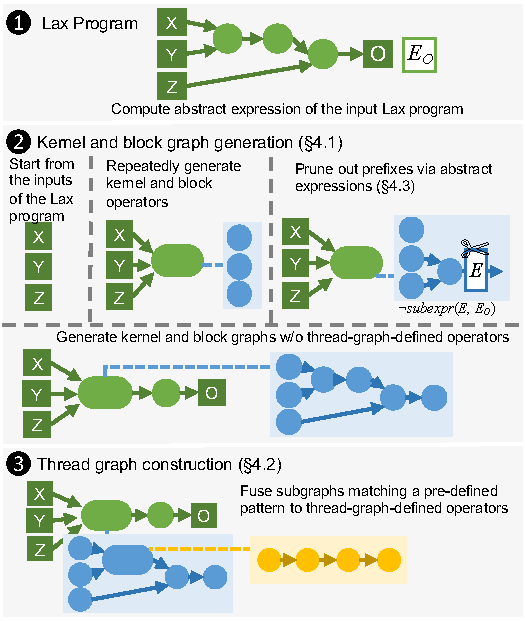
\includegraphics[width=\columnwidth]{figs/generator.pdf}
    \vspace{-1em}
    \caption{An overview of the \graph generator.}
    \vspace{\captionvspace}
    \label{fig:generator}
    % \vspace{\captionvspace}
\end{figure}

RMSNorm is often followed by a matrix multiplication (MatMul). \Cref{fig:rms_norm_baseline} shows the computation graph of an RMSNorm followed by a MatMul operator, where $X$ is the input tensor, and $G$ and $W$ denote two weight tensors.
Existing ML compilers generally launch two separate kernels for {RMSNorm} and MatMul computations, since both operations internally perform reductions across an input dimension, making it challenging to fuse their computations into a single kernel.
This approach requires storing intermediate results (i.e., $Y$) in device memory since different kernels cannot share data in shared memory or register files.

\Cref{fig:rms_norm_mlso} shows the best \graph automatically discovered by \sys for computing RMSNorm and MatMul in a single kernel. The computation is fused in a single graph-defined kernel operator to avoid saving intermediate results (i.e., $Y$) in device memory and reduce kernel launch overheads. 

We highlight the key differences between the \graph discovered by \sys and the original \graph.
These differences involve discovering new custom kernels and combining algebraic and schedule transformations, making it infeasible to discover the final \graph by separately considering algebraic and schedule transformations.
First, \sys reorders MatMul and the division of RMSNorm by leveraging the commutativity of matrix multiplication and element-wise division (algebraic transformation).
Second, \sys performs the accumulation in the root mean square (i.e., $A_i = \sum_j X_{ij}^2$) and the accumulation in the matrix multiplication (i.e., $B_{ik} = \sum_j X_{ij} G_j W_{jk}$) in parallel (schedule transformation), avoiding writing the accumulation results to device memory.
Next, \sys instantiates a thread graph to perform a sequence of element-wise operators while maintaining all intermediate results in register files (schedule transformation).
Finally, the best discovered \graph uses a new custom kernel to fuse the computation of RMSNorm and MatMul, reducing device memory access and kernel launch overheads. This \graph outperforms the hand-written kernels in existing systems by 1.5$\times$ and 1.9$\times$ on NVIDIA A100 and H100 GPUs respectively.
